\chapter{Architectures}
\label{chp:arch}

The following chapter will show and explain the different architectures used in this thesis.
The architectures were based on existing architectures used in the automotive industry.
While architectures used in the automotive industry are complex, with sometimes over 80 ECUs in one model, the architectures used in this thesis were sized down to a more manageable size, with ca. 20 ECUs for each architecture.
Each architecture was modeled using these components:

\begin{itemize}

    \item \textbf{ECUs}: The different ECUs in the architecture. They are the nodes of the graph.
    
    \item \textbf{Entry points}: The entry points to the architecture. The only possible entries are the external interfaces that an ECU might have.
    
    \item \textbf{Targets}: ECUs that are considered targets for an attacker. They are targets because they contain sensitive data or because they are critical for the vehicle's functionality.
    
    \item \textbf{Bus systems}: ECUs are connected to each other using bus systems. The bus systems are the edges in the graph. The possible bus systems are CAN, CANFD, LIN, FlexRay, and Ethernet.
    
    \item \textbf{Interfaces}: The interfaces are the connections between the ECUs and the external world. They are the connections between the ECUs and the bus systems. The possible interfaces are Bluetooth, Wifi, and Sattelite.
    
    \item \textbf{Attack feasibility}: Each component of the architecture (ECU, bus system, interface) has its own rating for its attack feasibility.

\end{itemize}

This thesis focuses on 13-15 architectures.
Ten architectures were used as a "training set" to determine and calibrate the criteria used to evaluate the remaining architectures, which are the focus of the comparison. 

\section{Training set architectures}
\begin{figure}
    \caption{Architecture 1}
    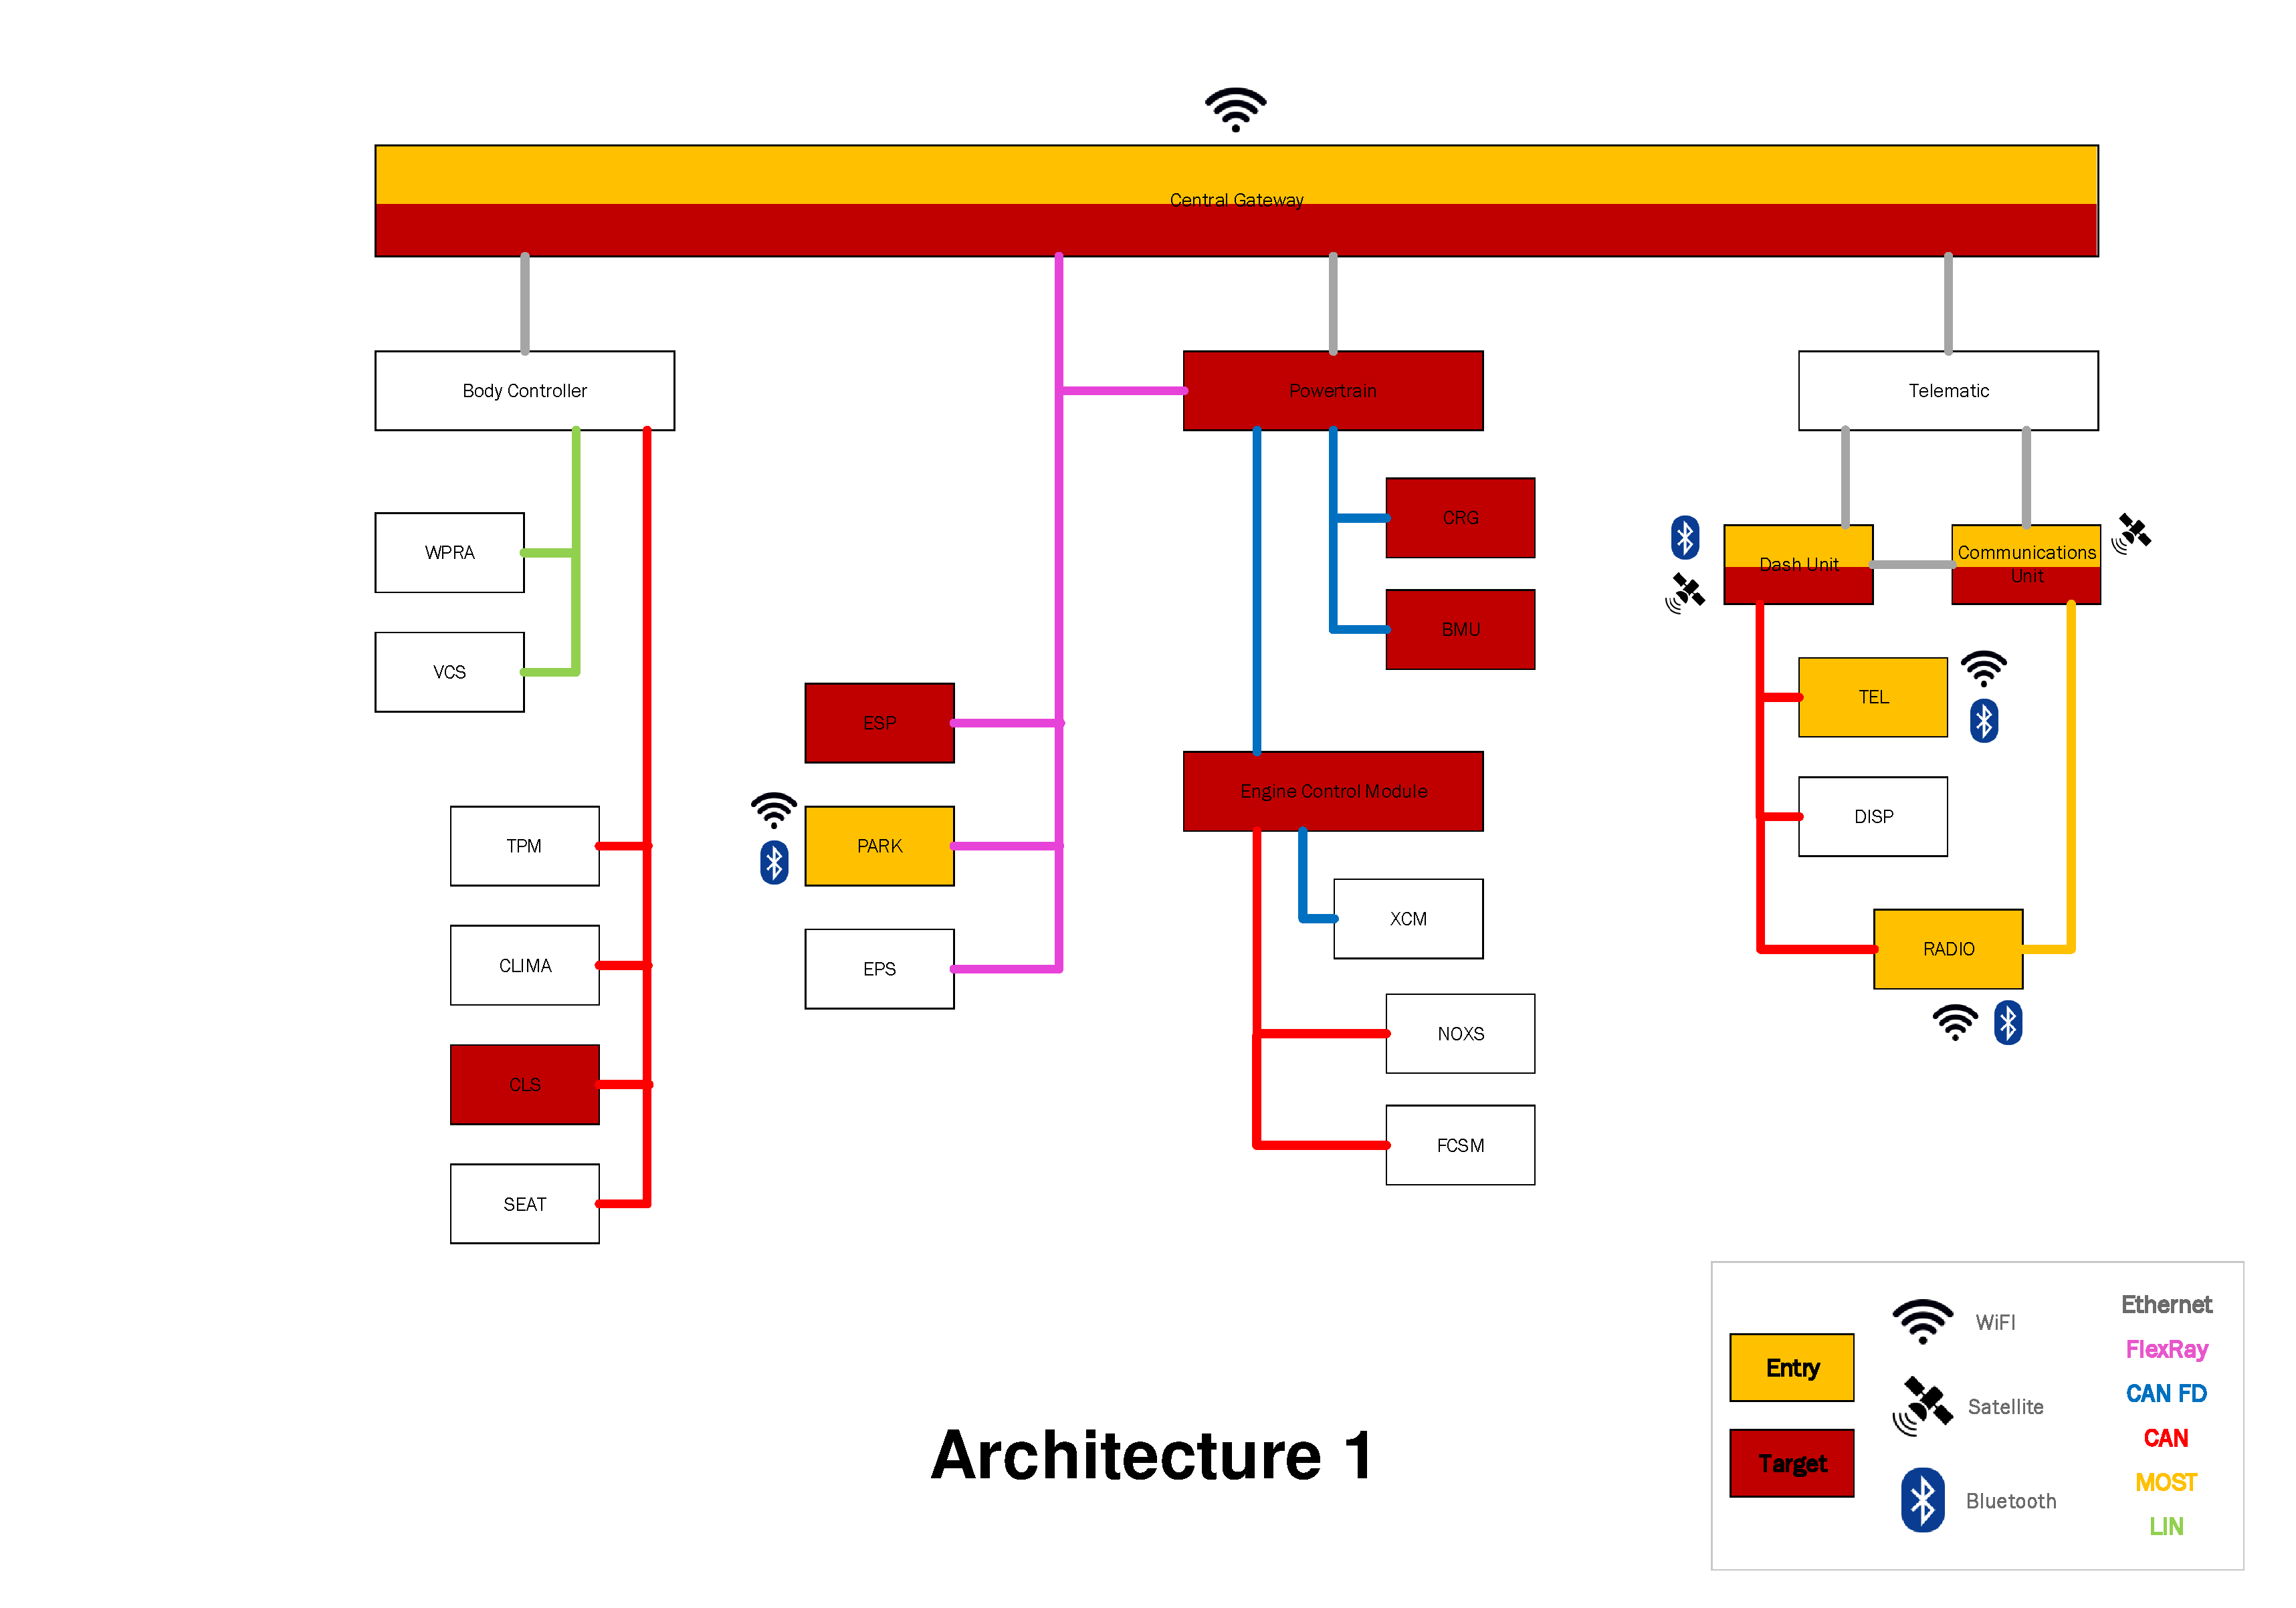
\includegraphics[width=\textwidth, page=1]{../Architectures-survey.pdf}
\end{figure}

\begin{figure}
    \caption{Architecture 2}
    \includegraphics[width=\textwidth, page=2]{../Architectures-survey.pdf}
\end{figure}

\begin{figure}
    \caption{Architecture 3}
    \includegraphics[width=\textwidth, page=3]{../Architectures-survey.pdf}
\end{figure}

\begin{figure}
    \caption{Architecture 4}
    \includegraphics[width=\textwidth, page=4]{../Architectures-survey.pdf}
\end{figure}

\begin{figure}
    \caption{Architecture 5}
    \includegraphics[width=\textwidth, page=5]{../Architectures-survey.pdf}
\end{figure}

\begin{figure}
    \caption{Architecture 6}
    \includegraphics[width=\textwidth, page=6]{../Architectures-survey.pdf}
\end{figure}

\begin{figure}
    \caption{Architecture 7}
    \includegraphics[width=\textwidth, page=7]{../Architectures-survey.pdf}
\end{figure}

\begin{figure}
    \caption{Architecture 8}
    \includegraphics[width=\textwidth, page=8]{../Architectures-survey.pdf}
\end{figure}

\begin{figure}
    \caption{Architecture 9}
    \includegraphics[width=\textwidth, page=9]{../Architectures-survey.pdf}
\end{figure}

\begin{figure}
    \caption{Architecture 10}
    \includegraphics[width=\textwidth, page=10]{../Architectures-survey.pdf}
\end{figure}